% Phase R1 (CP2-redo). Rewritten 2026-09-19 against WRITING_PLAN_2026-09-19.md v2.1 §5.2 and the
% rebuilt semantic.md §Method. Subsections are cut by component (model / learning / controller /
% guarantee), not one per design choice (D25). Equations are reused from the colleague's
% 3-method.tex; the outline, the opening and the Why paragraphs are not (D25).
\section{Method}
\label{sec:method}

A prompt and the reply it draws form one step of a dynamical system, and that
step is the clock used here. On a short window of verifier readings we
identify a command-conditioned Koopman dynamics model of that step. The model
then ranks candidate instructions before any of them is sent. The parameters
of $p_{\theta}$ never change, and the dynamics model is fit offline.
Figure~\ref{fig:method} shows one interaction step in both spaces on the
left and the controller built on the linear step on the right.

\begin{figure}[t]
    \centering
    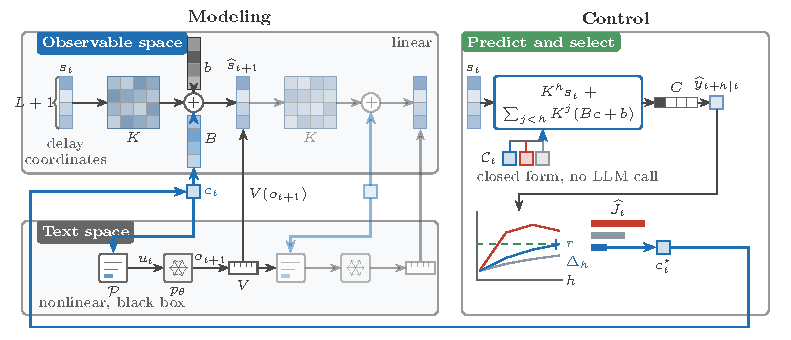
\includegraphics[width=\textwidth]{figs/method.pdf}
    \caption{Overview of KOMPAS. Left: one interaction step, seen in two
    spaces. In text space the frozen model turns a prompt into a reply and
    the verifier reads one attribute. In observable space the same step acts
    on the window of recent readings through the affine map, and the command
    $c_t$ enters both spaces from one cell. Right: the same operator's
    closed-form power rolls each candidate command forward, the predicted
    trajectories are scored against the target, and the best command returns
    as the next $c_t$. The operator is fit offline by least squares
    (Section~\ref{sec:learning}).}
    \label{fig:method}
\end{figure}

\subsection{A Koopman Dynamics Model of Prompt--Response Interaction}
\label{sec:model}

Three things decide the next reading. Part of it is carried forward by what
the recent turns have said. Part of it is pushed by the instruction issued
now. The rest is an offset the task holds fixed across the conversation. The
model below is the plainest map that keeps these three parts apart.

A single reading cannot say which way the conversation is moving. The same
sentence length can occur while successive revisions are becoming longer or
while they are becoming shorter. A memoryless rule issues the same command in
both situations, and the next step differs. Stacking the last several readings
separates the two, since the stack shows a level and a direction of travel. We
therefore represent the interaction by a finite window of attribute readings,
\begin{equation}
    s_t=
    \begin{bmatrix}
        y_t & y_{t-1} & \cdots & y_{t-L}
    \end{bmatrix}^{\top}
    \in\mathbb{R}^{L+1},
    \qquad
    y_t=C s_t,
    \label{eq:memory_state}
\end{equation}
Here $y_t$ is the measured attribute at step $t$
(Section~\ref{sec:problem_modeling}), $L\geq 1$ is the number of earlier
readings retained, and $C=[1,0,\ldots,0]$ reads the current attribute back out
of the stack. The vector $s_t$ is the memory state used in the rest of the
paper. A window of this kind is assumed to carry enough of the conversation to
predict the next reading. That is an approximation to the information
prediction needs, not a reconstruction of the dialogue state, and the
prediction experiments test it.

Before any approximation there is a population object to approximate. It is
the expected value of an observable one step ahead, given the current state
and the applied command. We write the command-conditioned Koopman operator
acting on an observable $f$ as
\begin{equation}
    (\mathcal{K}_{c}f)(s)
    =
    \mathbb{E}\!\left[
        f(s_{t+1})
        \mid s_t=s,\,c_t=c
    \right].
    \label{eq:koopman_operator}
\end{equation}
Here $\mathcal{K}_{c}$ is that operator, and it is linear in the observable
$f$ even where the prompt-response dynamics are not. The delay coordinates
stacked in $s_t$ are themselves a dictionary of observables. The affine model
stated below is the finite-dimensional approximation of $\mathcal{K}_{c}$ on
that dictionary.
% CITE: arbabi2017hankel, korda2018mpc

A command coordinate is available to the model because the prompt is built
from one. We fix a prompting protocol and draw every instruction from it,
\begin{equation}
    u_t=\mathcal{P}(x,\mathcal{H}_t,c_t),
    \qquad
    c_t\in\mathcal{C}\subseteq\mathbb{R},
    \label{eq:prompt_protocol}
\end{equation}
Here $\mathcal{P}$ builds a prompt from the task input $x$, the dialogue
history $\mathcal{H}_t$ of Section~\ref{sec:problem_modeling} and a numerical
command $c_t$, and $\mathcal{C}$ is the range of admissible commands. The
coordinate is a property of the protocol that generates the instruction,
rather than of the instruction's surface wording. The treatment therefore
covers instructions from this protocol, not text inputs with an unspecified
encoding.

With a state and a command coordinate in place, the three-part map of the
opening paragraph has one plain form,
\begin{equation}
    \widehat{s}_{t+1}
    =
    K s_t+B c_t+b,
    \qquad
    \widehat{y}_{t+1}
    =
    C\widehat{s}_{t+1}.
    \label{eq:koopman_model}
\end{equation}
Here $K\in\mathbb{R}^{(L+1)\times(L+1)}$ carries the window forward,
$B\in\mathbb{R}^{(L+1)\times 1}$ is the column through which one unit of
command acts, and $b\in\mathbb{R}^{L+1}$ is a bias. Two restrictions are imposed
here by choice. One transition is shared by all commands, and the command
enters through one column. Neither follows from the operator being linear, and
no exact finite-dimensional Koopman representation of $p_{\theta}$ is assumed.

One generalization is worth naming, since a Koopman model is often written on
features of the state rather than on the state itself. A lifting is a change of
coordinates. The same affine step is written on learned features
$E_{\phi}(s_t)$ of the window instead of on the window, and a decoder maps
those features back. One reason to reach
for one is familiar from regression: the right features let a straight line
fit a curved relation. A curved one-step map behaves the same way. This
paper reports the identity lifting, which leaves the model written on the
readings themselves; the learned variant is kept as a comparison row and is
trained as in Appendix~\ref{app:A1_estimator}. A reading here is one scalar
and the window is short, which leaves learned features little extra structure
to expose.

\textbf{Why a Linear Operator on a Short Window Can Carry Multi-Turn
Dynamics.} Written out, the reported instance is a delay regression with an
exogenous input, and a reader is entitled to ask what the operator view adds.
One thing it adds belongs to that view alone. The operator acts on
observables, so a learned lifting is a change of dictionary inside one model
rather than a second model. The linear instance is that same dictionary, left
as it is. Two further properties this section leans on come with any affine
state-space form: the multi-step forecast has a closed form, and a planner can
consume that forecast. \uline{The operator view buys no accuracy of its own,
and it is what puts the raw window, the learned features and the planner into
one family.}

\subsection{Learning the Model from Interaction Data}
\label{sec:learning}

The training data is a set of recorded transitions. Each window of $L+1$
readings supplies one state, and sliding the window by one step supplies the
next transition. The command label of a transition is the command applied
before the successor reading. For a trajectory recorded under one fixed
requested target, that target labels every step of the trajectory.

In the reported instance the unknowns are the transition, the command column
and the bias. All three enter the next-step prediction linearly, which makes
fitting them to the recorded transitions a least-squares problem,
\begin{equation}
    (\widehat{K},\widehat{B},\widehat{b})
    =
    \operatorname*{arg\,min}_{K,B,b}
    \sum_{t}
    \bigl\|
        s_{t+1}-(K s_t+B c_t+b)
    \bigr\|_2^2 .
    \label{eq:identification}
\end{equation}
The sum runs over every transition $(s_t,c_t,s_{t+1})$ that the overlapping
windows of the training trajectories supply, with $s_{t+1}$ the recorded
successor state. The problem admits a closed-form solution. For the window
lengths used here the unknown entries number in the tens, which keeps the
count of unknowns small next to the count of recorded transitions.

What the training trajectories cover decides where the fitted model can be
trusted. Accurate prediction on trajectories with a fixed command does not by
itself establish accuracy after a command changes. The reliable range at
inference time is therefore set by the command-history pairs the training
trajectories contain.

The learned-lifting variant replaces the identity map with an encoder and fits
it together with the transition under a three-term objective.
Appendix~\ref{app:A1_estimator} states that objective; what a lifting is was
said above.

\subsection{Predictive Instruction Selection with Replanning}
\label{sec:controller}

\textbf{Why Scoring Happens Without Opening the Model.} A candidate has to be
judged before it is sent, and the judge cannot look inside the model that
would answer it. The score therefore reads only the attributes a candidate is
predicted to produce. Nothing internal to the generator enters the comparison,
and nothing beyond one instruction is asked of the interface. \uline{A
candidate is judged only by the reply attributes it is predicted to produce,
never by anything inside the model that would produce them.}

Evaluating a candidate means holding its command fixed over a lookahead and
rolling the state forward, with no further generation from the frozen model.
Let $\mathcal{C}_t\subseteq\mathcal{C}$ be the finite nonempty candidate set
at step $t$, and let the rollout start from the observed window,
\begin{equation}
    \begin{aligned}
        \widehat{s}_{t\mid t}(c)
        &= s_t,\\
        \widehat{s}_{t+h\mid t}(c)
        &=
        K\widehat{s}_{t+h-1\mid t}(c)+Bc+b,\\
        \widehat{y}_{t+h\mid t}(c)
        &=
        C\widehat{s}_{t+h\mid t}(c),
        \qquad h=1,\ldots,H.
    \end{aligned}
    \label{eq:rollout}
\end{equation}
Here $\mathcal{C}_t$ is the candidate set the controller ranks at this step,
and $H$ is the prediction horizon in interactions, truncated to the remaining
interaction budget. What that set holds is a property of the task rather than
of the controller: a finite list of admissible command values, fixed before
the loop begins.
% TODO(data): the per-benchmark candidate lists are part of the colleague's control setup and
% are reported with the experiments, not here.

An affine transition with the command in one column turns an $h$-step
lookahead into a matrix power. The rollout then has the explicit form
\begin{equation}
    \widehat{s}_{t+h\mid t}(c)
    =
    K^h s_t
    +
    \sum_{j=0}^{h-1}K^j(Bc+b).
    \label{eq:closed_form_rollout}
\end{equation}
Evaluating one candidate costs a matrix product and a readout. It adds no
query to $p_{\theta}$, whatever the size of the candidate set.

A candidate is scored on its whole predicted trajectory, not on its immediate
effect. That lets the controller issue a command different from the target
while the attribute is still moving. Each candidate is scored by its predicted
deviation from the desired attribute,
\begin{equation}
    \begin{aligned}
        \widehat{J}_t(c)
        &=
        \sum_{h=1}^{H}w_h
        \left|
            \widehat{y}_{t+h\mid t}(c)-r
        \right|^2,\\
        c_t^{\star}
        &\in
        \operatorname*{arg\,min}_{c\in\mathcal{C}_t}
        \widehat{J}_t(c),
        \qquad w_h\geq 0.
    \end{aligned}
    \label{eq:selection}
\end{equation}
Here $w_h$ is the weight on the deviation $h$ steps ahead. The quantity
$\widehat{J}_t$ is the predicted cost of holding one command over the horizon,
and $c_t^{\star}$ is the command that minimizes it.

\begin{algorithm}[ht]
\caption{The receding-horizon loop that runs at inference time. Inputs: the frozen
$p_{\theta}$, the fitted $(K,B,b)$, the protocol $\mathcal{P}$, the reference $r$, the horizon
$H$, and an interaction budget $T$.}
\label{alg:loop}
\begin{enumerate}
    \item Read the attribute $y_t=V(o_t)$ of the reply in hand.
    \item Shift $y_t$ into the window to form the state $s_t$.
    \item For each candidate $c\in\mathcal{C}_t$, roll $s_t$ forward over $H$ steps by
          \eqref{eq:closed_form_rollout} and score $\widehat{J}_t(c)$.
    \item Take $c_t^{\star}\in\operatorname*{arg\,min}_{c\in\mathcal{C}_t}\widehat{J}_t(c)$.
    \item Send $u_t=\mathcal{P}(x,\mathcal{H}_t,c_t^{\star})$ and receive the reply $o_{t+1}$.
    \item Return to step 1 until the budget $T$ is spent.
\end{enumerate}
\end{algorithm}

The controller executes the first step of a plan and no more of it. The new
reading, not a predicted one, is what the next plan starts from. A command
held constant belongs to the hypothetical rollout, never to the executed
sequence. Candidate simulation adds no query to the target model, and building
candidates and reading replies still count against the interaction budget.

\subsection{What Prediction Accuracy Buys}
\label{sec:guarantee}

An accurate model is worth having because it makes the selected command hard
to improve on in hindsight. For a candidate $c$, let $y_h^c$ be the attribute
reached after $h$ interactions that hold $c$. Let
$J_t(c)=\sum_{h=1}^{H}w_h|y_h^c-r|^2$ be the cost those readings incur. The
next statement bounds the gap between that cost and the smallest one on
offer.
\begin{proposition}[Selection error under bounded residuals]
\label{prop:selection}
Suppose that over the candidate rollouts the one-step state residual stays
below $\varepsilon_{\mathrm{dyn}}$ and the readout residual stays below
$\varepsilon_{\mathrm{rec}}$. Suppose the readout does not amplify small state
differences without bound. Then
\begin{equation}
    \left|
        y_h^c-\widehat{y}_{t+h\mid t}(c)
    \right|
    \leq
    \Delta_h,
    \qquad h=1,\ldots,H,
    \label{eq:prediction_bound}
\end{equation}
and the selected command satisfies
\begin{equation}
    J_t(c_t^{\star})
    \leq
    \min_{c\in\mathcal{C}_t}J_t(c)+2\delta_J.
    \label{eq:selection_bound}
\end{equation}
\end{proposition}
Here $\Delta_h$ is the $h$-step attribute error bound, which accumulates the
one-step residual $\varepsilon_{\mathrm{dyn}}$ over $h$ steps and adds the
readout residual $\varepsilon_{\mathrm{rec}}$. The quantity $\delta_J$
accumulates $\Delta_h$ over the horizon weights and bounds the gap between a
candidate's predicted and actual held-command cost.
Appendix~\ref{app:A6_selection_bound} gives both in closed form.

The proof is two short steps. Predicted and actual rollouts start from the
same window, so their gap grows only through the accumulated one-step
residual. Applying the cost bound on either side of the minimizing choice
gives the factor of two.

The statement compares candidates under one held command. It does not promise
that $\mathcal{C}_t$ holds a command able to reach $r$, and it does not
promise that the replanned loop converges. Re-observation resets the initial
error of the next rollout and removes neither model mismatch nor the limits of
the candidate set. \uline{Rollouts that stay accurate keep the selected
candidate's cost within twice the best achievable estimation error, for this
one held-command comparison.}
